\documentclass[11pt,a4paper,english]{article}
  \usepackage[latin1]{inputenc}
  \usepackage{amsmath,amsfonts,amssymb}
  \usepackage{enumitem}
  \usepackage{fullpage}
  \usepackage{graphicx}
  \usepackage{tabto}
  \usepackage{etoolbox}
  \usepackage{hyperref}
  \usepackage{minted}
  \usepackage{parskip}
  \usepackage[font=small,labelfont=bf]{caption}
  \newcommand\numberthis{\addtocounter{equation}{1}\tag{\theequation}}
  \renewcommand{\labelenumii}{\theenumii}
  \renewcommand{\theenumii}{\theenumi.\arabic{enumii}.}

  \title{Algorithmic Methods of Data Mining - Assignment 2}
  \author{Maksad Donayorov}

  \begin{document}
    \maketitle
    \definecolor{bg}{rgb}{0.95,0.95,0.95}

    \section{Problem. \textit{Clustering given a hierarchy:}}
      \subsection{
        \textit{k-means on trees can be solved optimally in polynomial time}
      }
        To prove the k-means on tree can be solved optimally in polynomial time let's start by stating a pseudocode that solves this problem and then discuss how it works:
        \begin{minted}[bgcolor=bg,linenos,fontsize=\small,autogobble]{python}
          optimal_clusters = []
          for node in TraversalPostorder(tree):
            if node does not have children:
              tuple = (1, 0, [node.index], [node.value])
              optimal_clusters.append(tuple)
            if node has children:
              children = node.left_child + node.right_child
              numb_of_clusters = children.clusters
              node_self = (
                numb_of_clusters,
                calc_self_var,
                [children.indices],
                [children.elements]
              )
              tuple = (node_self, children)
              optimal_clusters.append(tuple)
            tuple.filter_the_optimal
          tuple.trim_elements
        \end{minted}

        Assume that we have a tree like this:
        \begin{minted}[bgcolor=bg,fontsize=\small,autogobble]{text}
               1
             /   \
            2     3
          /   \
         4     5
        \end{minted}
        Then the $TraversalPostorder(tree)$ will run as:
        \begin{minted}[bgcolor=bg,fontsize=\small,autogobble]{text}
          4 5 2 3 1
        \end{minted}

        This allows us to travel through the tree only once. Based on the pseudocode we should not need to refer to the children once we have computed the needed parameters. The main idea in here is that we create a $tuple$ of the needed parameters once we are visiting a node or a leaf, store all of the parameters and move to the next. For instance, at line 4:
        \begin{minted}[bgcolor=bg,fontsize=\small,autogobble]{python}
          tuple = (1, 0, [node.index], [node.value])
        \end{minted}
        We ar creating the tuple out of a leaf. The first parameter of that $tuple$ is an indicator of clusters and since a leaf can only have a cluster of one element, it's default value is 1. \\
        The second parameter of that tuple is $0$, that indicates the variance at that point. Again, since there is no more than one element at the leaf the variance will be $0$. \\
        The third element is an array of indices, we need that the very end and I will explain this later. \\
        The fourth parameter is the an array of element that that leaf holds. This will be needed once we aren in the parent node and want to compute the variance.\\
        After we do the computation at the first leaf we move to the next leaf and eventually to the parent where we compute the parameters (later in the example these parameters are noted as tuples).
        This sounds very complicated and indeed it is, as there isn't a better approach I came up with. Let's look into more concrete example hope to make things more clear. Let's assume that we have this tree with given leaves:
        \begin{minted}[bgcolor=bg,fontsize=\small,autogobble]{text}
                v1
              /   \
            v2     v3
           /  \   /  \
          2    4 v4   \
                /  \   \
               3   7   12
        \end{minted}

        In this tree we have $n=5$ and the leaves are 2, 4, 3, 7, 12. We have 4 "layers" and we can compute the variance, number of clusters and number of vertices. The first thing we do is to compute the level $I$ as that's the easiest (please note that we are not following at this point the postorder's steps). This is how it looks like:
        \begin{center}
          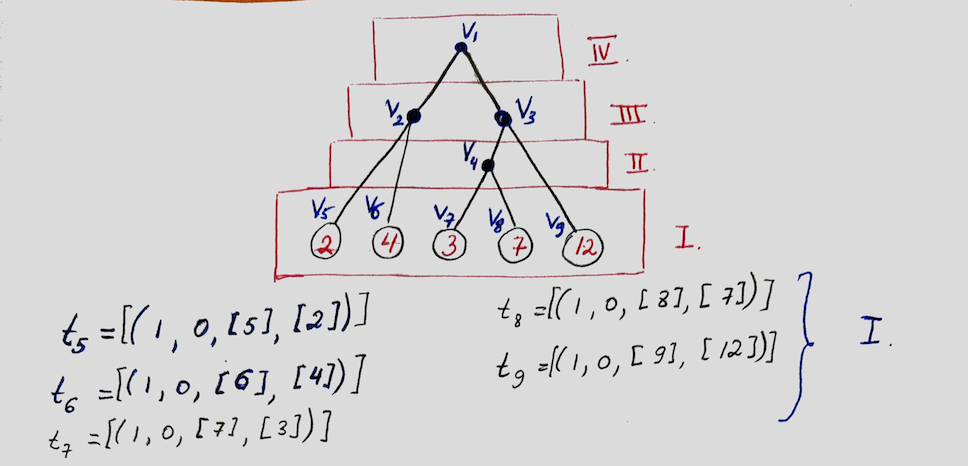
\includegraphics[width=15cm]{sc_1.png}
        \end{center}
        Here we create tuples for each leaf. For example, the:
        \begin{minted}[bgcolor=bg,fontsize=\small,autogobble]{python}
          t5 = (1, 0, [5], [2])
        \end{minted}

        means that this is the vertex 5, that has one "cluster", it's index is 5 and the elements that it holds are [2]. With that representation we can move to the second and third "levels". \\
        It is a bit tricky to calculate the tuples for nodes. That's because the nodes have 2 combinations:
        \begin{enumerate}
          \item When we are clustering the elements in the node (let's denote it by $t_{self}$).
          \item When we are clustering the elements in the children nodes/leaves ($t_{left} + t_{rigth}$).
        \end{enumerate}

        Let's now calculate the parameters ($t_2$) for $vertex_2$:
        \begin{center}
          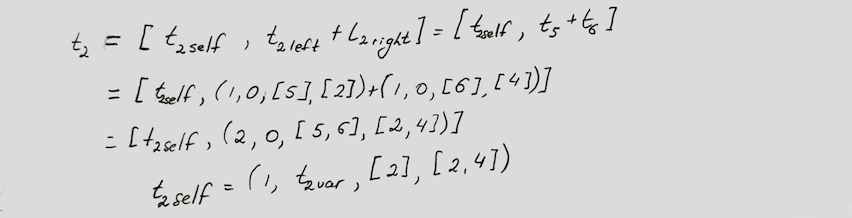
\includegraphics[width=15cm]{sc_2.png}
        \end{center}

        Now that we have calculated the left and the rigth children of $t_2$, we need to find the variance at $t_2$ that will be used for $t_{self}$:
        \begin{center}
          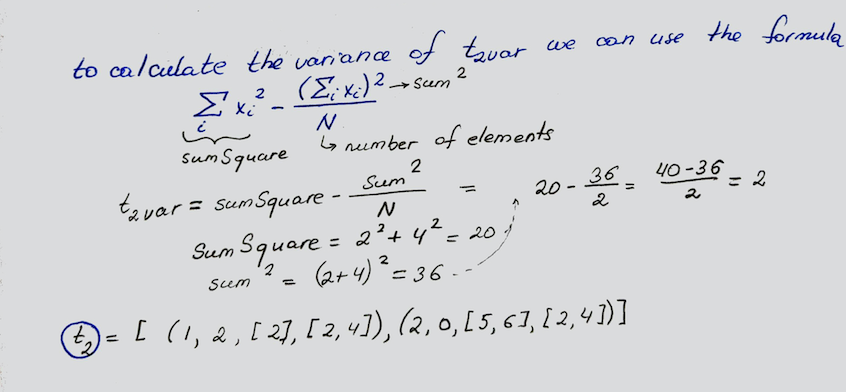
\includegraphics[width=15cm]{sc_3.png}
        \end{center}

        As you might have noticed we are not using the formula that is given in the problem description to calculate the variance (\href{https://math.stackexchange.com/questions/20593/calculate-variance-from-a-stream-of-sample-values}{link to the formula}). Instead, we are using a more efficient formula that relies on number of elements, sum of the elements and "square sum" of those elements.

        Now we can move to the next vertex and certainly the same logic applies:
        \begin{center}
          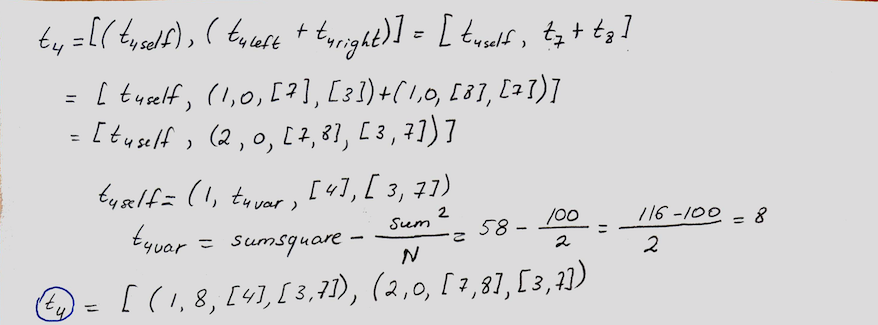
\includegraphics[width=15cm]{sc_4.png}
        \end{center}

        Please pay attention to the summation of left and right children that have more than one tuple:
        \begin{center}
          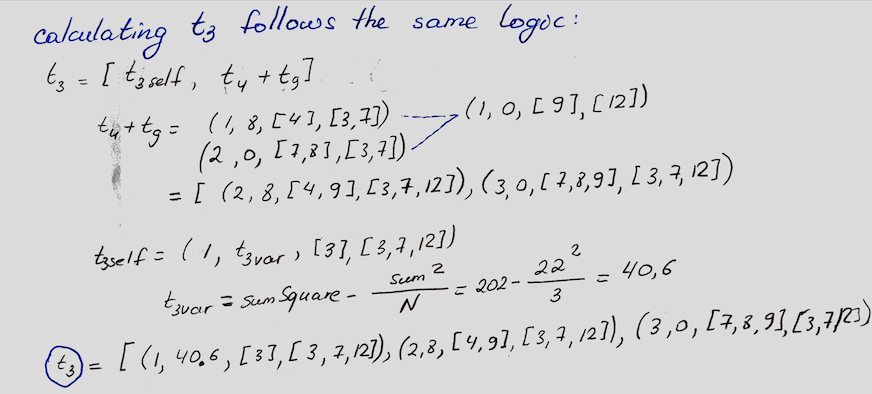
\includegraphics[width=15cm]{sc_5.png}
        \end{center}

        Up to this point we have computed all the parameters (tuples) for the all the children. Now, it's time to calculate them for $vertex_1$.
        \begin{center}
          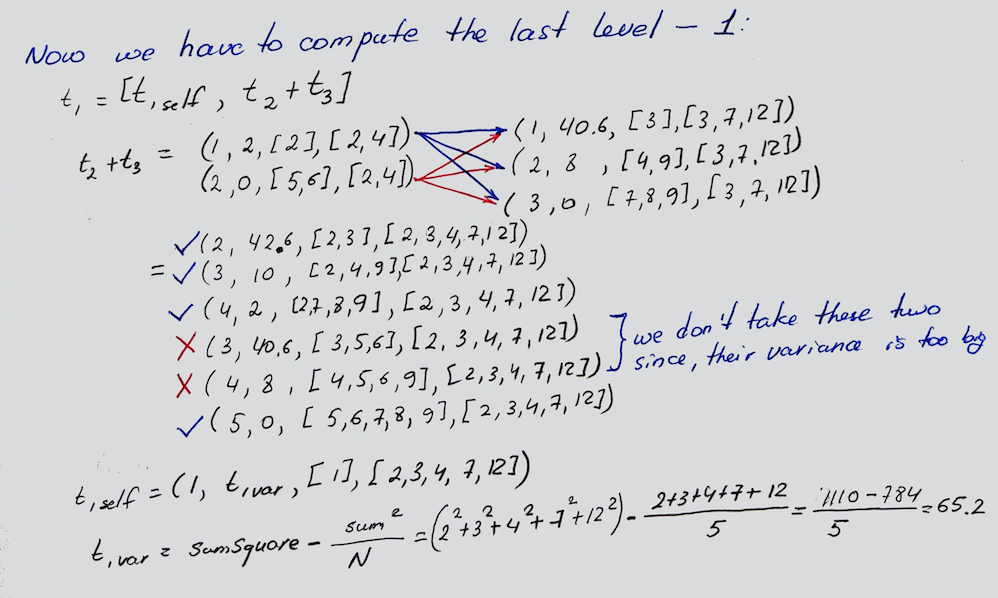
\includegraphics[width=15cm]{sc_6.png}
        \end{center}
        A very important point in the above calculation is how we choose some of the tuples. As you can see, those tuples that we choose are marked with the blue tick and those which are not chosen marked by red cross. This implies that we have 2 clusters with the same value of $k$ and we only choose the optimal one, which is a tuple with the smaller variance. In the pseudocode that's done on line 16.

        The final version of the $t_1$ looks like this:
        \begin{center}
          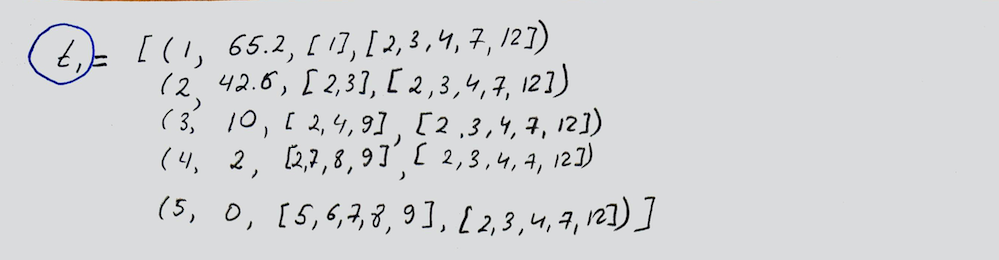
\includegraphics[width=15cm]{sc_7.png}
        \end{center}

        The final result that our algorithm returns is a list of the tuples with all the possible combination of clusters where $1 \leq k \leq 5$. Looking at this table we can immoderately tell what is the optimal cluster, what kind of vertices it will have and what is its variance (the elements are that each tuple holds are trimmed at line 17 of the pseudocode):
        \begin{minted}[bgcolor=bg,fontsize=\small,autogobble]{text}
          [
            (1, 65.2, [1],           ),
            (2, 42.6, [2, 3],        ),
            (3, 10,   [2, 4, 9],     ),
            (4, 2,    [2, 7, 8, 9],  ),
            (5, 0,    [5, 6, 7, 8, 9])
          ]
        \end{minted}

        For example, if $k=3$, we can say that the optimal cluster will have variance of $10$ with vertices indices of [2, 4, 9]:
        \begin{minted}[bgcolor=bg,fontsize=\small,autogobble]{text}
               v1
              /   \
            v2     v3
                  /  \
                 v4   12
        \end{minted}

        Or if $k=4$, then the optimal cluster will have a variance of 2 with vertices [2, 7, 8, 9]:
        \begin{minted}[bgcolor=bg,fontsize=\small,autogobble]{text}
                v1
              /   \
            v2    v3
                 /  \
                v4   \
               /  \   \
              3    7  12
        \end{minted}

      \subsection{
        \textit{correctness of this algorithm}
      }

      \subsection{
        \textit{complexity of the algorithm}
      }
\end{document}

